%!TeX program = xelatex
%Do not change
\documentclass[12pt, oneside]{article}
\usepackage{amssymb,amsmath}
\usepackage[margin=1in]{geometry}
\usepackage{textpos}
\usepackage{float}
\usepackage{booktabs}
%\usepackage{color}
\usepackage{graphicx}
\usepackage[inter-unit-product =\cdot]{siunitx}
\let\DeclareUSUnit\DeclareSIUnit
\let\US\SI
\DeclareUSUnit\inch{in}
\DeclareUSUnit\foot{ft}
\DeclareUSUnit\mile{mi}
\DeclareUSUnit\foot{ft}
\DeclareUSUnit\slug{slug}
\DeclareUSUnit\pound{lb}
\DeclareUSUnit\psi{psi}
\DeclareUSUnit\Msi{Msi}
\DeclareUSUnit\ksi{ksi}

%\usepackage{tikz}
%\usetikzlibrary{positioning}
%\usepackage{tikz-3dplot}
%\usepackage{pgfopts}
%\usepackage{wasysym}
%\usepackage{stanli}

% You may add the packages you need here
\begin{document}

%TODO change numbers in problems
\begin{textblock*}{4cm}(-1.7cm,-2.3cm)
\noindent {\scriptsize AE333 Spring 2021}
\end{textblock*}

%Do not modify other than putting your name where stated
\begin{textblock*}{8cm}(12.5cm,-1cm)
\noindent {Name: }
\end{textblock*}
%Do not modify other than typing your acknowledgement where stated
\begin{textblock*}{13.5cm}(-1.7cm,-1.8cm)
%\noindent \textit{\footnotesize Acknowledgement: Your acknowledgement for collaboration and other sources goes here. }
\end{textblock*}

\vspace{1cm}

%Do not modify other than typing the homework number after #
\begin{center}
\textbf{\Large Homework 6}

\textbf{Due 29 March 2021}
\end{center}

\begin{enumerate}
	\item %F7-2
		Find the shear stress at points $A$ and $B$ when $V = 	\SI{450}{kN} $.
		Draw the state of stress on a volume element at each point.
		\begin{figure}[H]
			\centering
			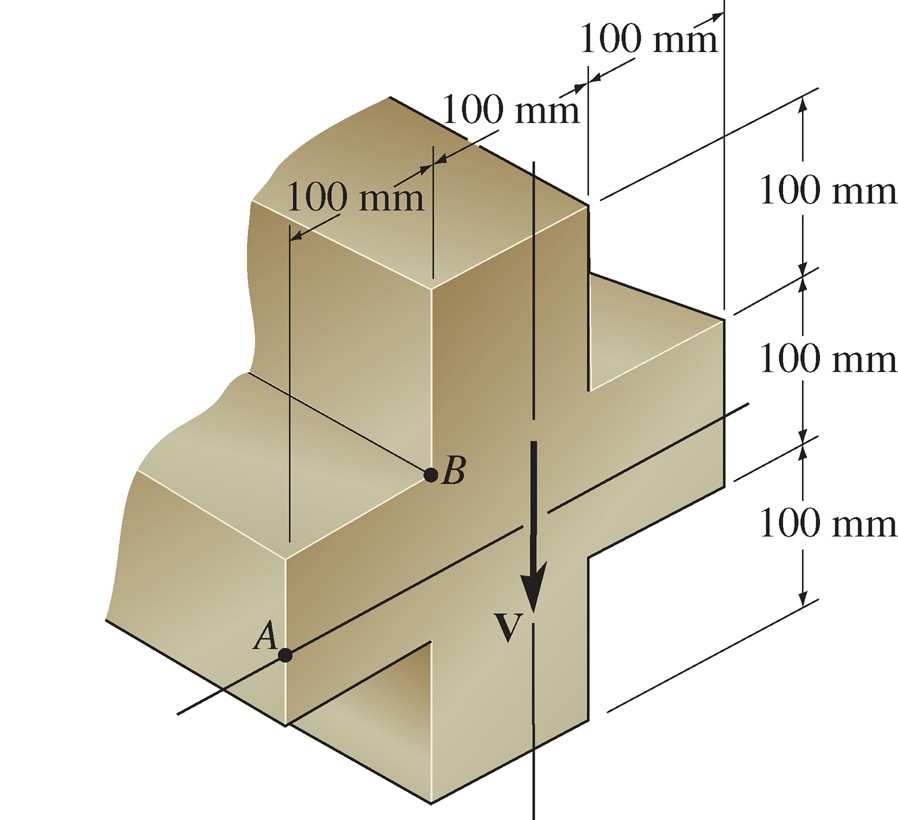
\includegraphics[width=0.6\linewidth]{f7-2}
		\end{figure}
	\item %7-25
		Find the maximum shear stress acting on the beam shown.
		\begin{figure}[H]
			\centering
			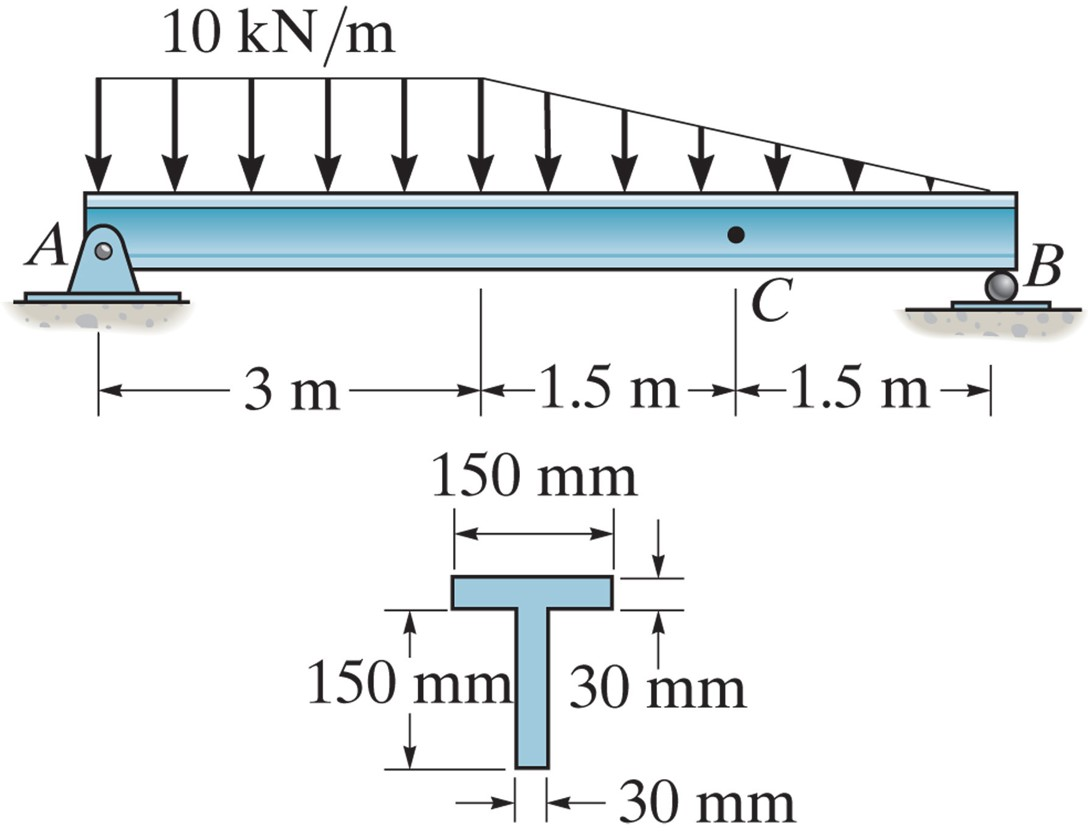
\includegraphics[width=0.6\linewidth]{7-25}
		\end{figure}
	\item %7-11
		The overhanging beam is subjected to a uniform load of $w= 	\SI{75}{kN/m} $.
		Find the maximum shear stress in the beam.
		\begin{figure}[H]
			\centering
			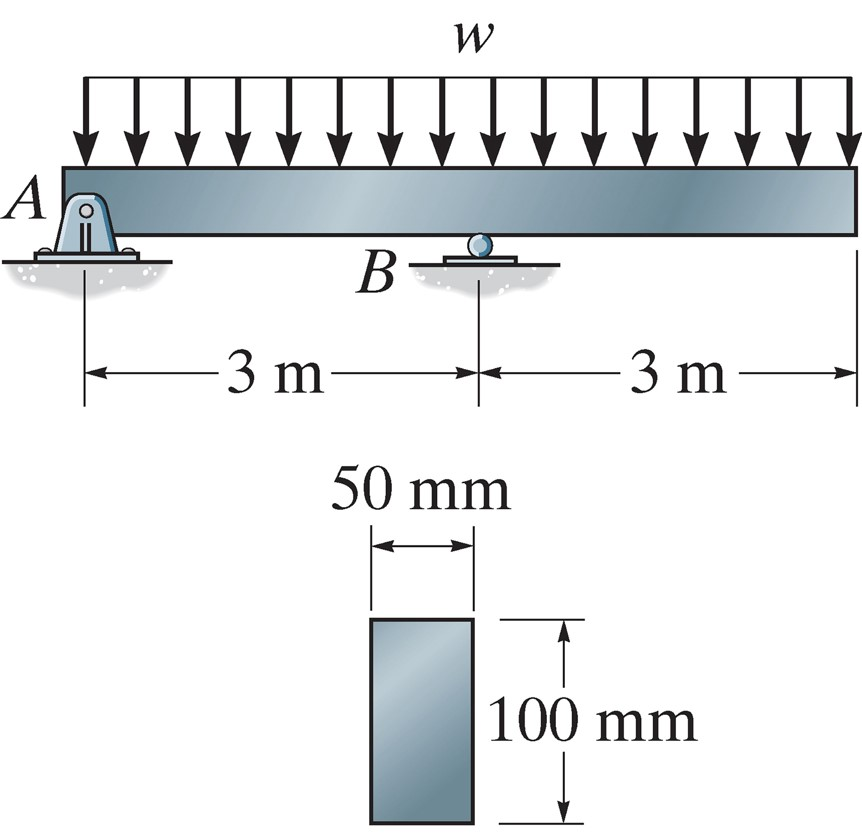
\includegraphics[width=0.5\linewidth]{7-11}
		\end{figure}
	\item %F7-7
		Two identical $ 	\SI{20 }{mm}  $ plates are bolted to the top and bottom of a flange to form a built-up beam.
		For a shear force of $V = 	\SI{400 }{kN} $ find the maximum bolt spacing, $s$, if each bolt has a shear strength of $ 	\SI{45 }{kN}  $
		\begin{figure}[H]
			\centering
			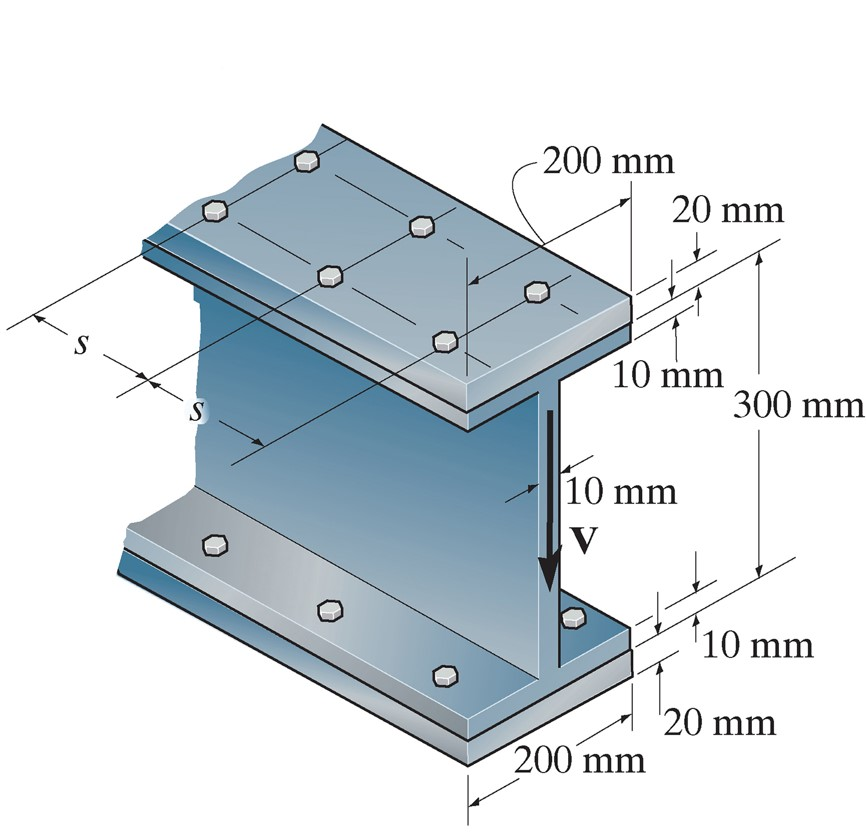
\includegraphics[width=0.6\linewidth]{f7-7}
		\end{figure}
		\newpage
	\item %7-46
		The beam shown is made by gluing two $ 	\US{1/2 }{in}  $ c-channel strips together as sown.
		If the glue has a maximum shear stress of $\tau = 	\US{600}{psi} $ find the maximum intensity, $w_0$, of the triangular distributed loading.
		\begin{figure}[H]
			\centering
			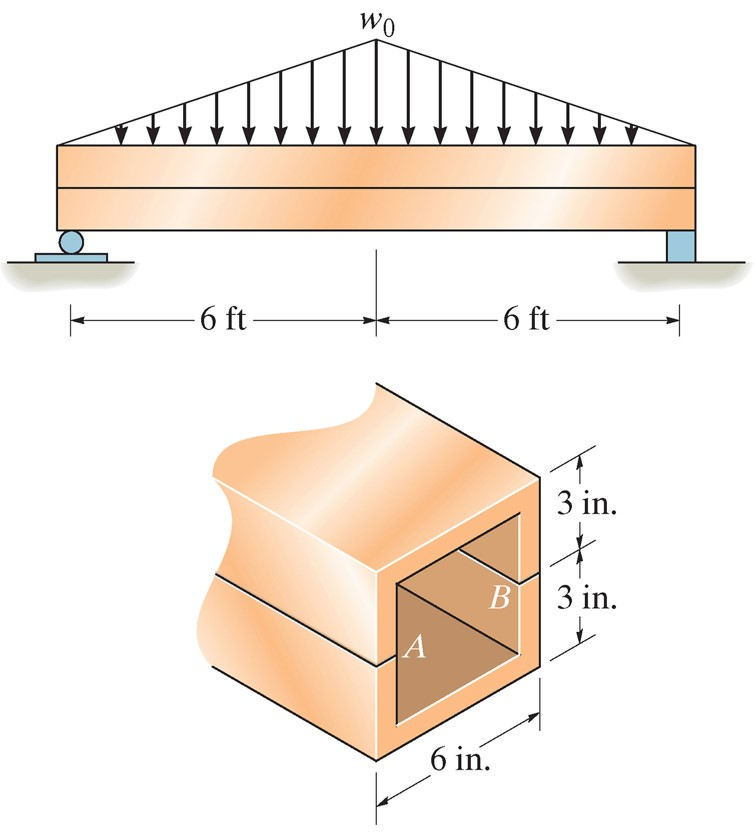
\includegraphics[width=0.6\linewidth]{7-46}
		\end{figure}

\end{enumerate}
\end{document}
